\documentclass{beamer}
\usepackage{listings}
\lstset{
%language=C,
frame=single, 
breaklines=true,
columns=fullflexible
}
\usepackage{amsthm}
\usepackage{mathtools}
\usepackage{blkarray}
\usepackage{subcaption}
\usepackage{url}
\usepackage{tikz}
\usepackage{enumitem}
\usepackage{tkz-euclide} % loads  TikZ and tkz-base
%\usetkzobj{all}
\usetikzlibrary{calc,math}
\usepackage{float}
\newcommand{\myvec}[1]{\ensuremath{\begin{pmatrix}#1\end{pmatrix}}}
\providecommand{\brak}[1]{\ensuremath{\left(#1\right)}}
\newcommand\norm[1]{\left\lVert#1\right\rVert}
\renewcommand{\vec}[1]{\mathbf{#1}}
\usepackage[export]{adjustbox}
\usepackage[utf8]{inputenc}
\usepackage{amsmath}
\usepackage{physics}
\usepackage{tikz}
\usetikzlibrary{automata, positioning}
\usetheme{Boadilla}
\providecommand{\pr}[1]{\ensuremath{\Pr\left(#1\right)}}

\title{ASSIGNMENT 3}
\author{ANANTHOJU PRANAV SAI - AI20BTECH11004}
\begin{document}
\begin{frame}
\titlepage
\end{frame}
\begin{frame}{Question}
    \begin{block}{Construction 2.11}
    Construct PLAN where PL = 4, LA = 6.5, $\angle$P = 90$^\circ$,$\angle$A = 110$^\circ$ and $\angle$N=85$^\circ$
    \end{block}
\end{frame}
\begin{frame}
\begin{lemma}
    Let ABCD be a quadrilateral with 
    \begin{align}
        \norm{B-A} = a\\
        \norm{C-B} = b\\
        \angle A = \theta\\
        \angle C = \beta\\
        \angle D = \gamma\\
        \vec{A} = \myvec{0\\
                         0}\\
        \vec{B} = \myvec{a\\
                         0}   
    \end{align}
\end{lemma}
\end{frame}
\begin{frame}
\begin{block}{Lemma contd..}
    then the remaining vectors can be found using 
    \begin{align}
        \vec{C} = \vec{B}+b\myvec{\cos{(180-\alpha)}\\
                                  \sin{(180-\alpha)}}
    \end{align}
    where $\alpha$ = $360-(\theta+\beta+\gamma)$
    \begin{align}
        \vec{D} = d\myvec{\cos{\theta}\\
                          \sin{\theta}}
    \end{align}
    where 
    \begin{align}
        d &= \norm{A-D} = e\times\brak{\frac{\sin{\brak{\beta-\sin^{-1}\brak{{\frac{a\sin\alpha}{e}}}}}}{\sin\gamma}}\\
        e &= \norm{C-A} = \sqrt{a^2+b^2-2ab\cos{\alpha}}
    \end{align}
\end{block}
\end{frame}
\begin{frame}
\begin{proof}
    Let,
    \begin{align}
        \angle {ACB} = \beta_1\\
        \angle {ACD} = \beta_2\\
        \implies \beta_1 + \beta_2 = \beta \label{a}
    \end{align}
    Now in $\triangle$ ABC applying cosine rule gives,
    \begin{align}
        e &= \sqrt{a^2+b^2-2ab\cos{\alpha}}
    \end{align}
    and in $\triangle$ ABC applying sine rule gives,
    \begin{align}
        \frac{\sin{\angle{ACB}}}{AB} = \frac{\sin B}{AC}\\
        \implies \frac{\sin{\beta_1}}{a} = \frac{\sin{\alpha}}{e}\\
        \implies \beta_1 = \sin^{-1}\brak{\frac{a\sin\alpha}{e}}   \label{b}     
    \end{align}
\end{proof} 
\end{frame}
\begin{frame}
\begin{block}{Proof cont..d}
    and in $\triangle$ ACD applying sine rule gives,
    \begin{align}
        \frac{\sin{\angle{ACD}}}{AD} &= \frac{\sin D}{AC}\\
        \implies \frac{\sin{\beta_2}}{d} &= \frac{\sin{\gamma}}{e}\\
        \implies d &= e\times\brak{\frac{\sin{\brak{\beta-\sin^{-1}\brak{{\frac{a\sin\alpha}{e}}}}}}{\sin\gamma}}
    \end{align}
\end{block}
\end{frame}
\begin{frame}{Solution}
Given, 
\begin{align}
    \angle P &= 90^\circ = \theta\\
    \angle A &= 110^\circ = \beta\\
    \angle N &= 85^\circ = \gamma\\
    \implies \angle L &= 75^\circ = \alpha\\
    \norm{\vec{L}-\vec{P}} &= 4 = a\\
    \norm{\vec{A}-\vec{L}} &= 6.5 = b\\
    &\vec{P} = \myvec{0\\
                     0}\\
    &\vec{L} = \myvec{4\\
                      0}
\end{align}
\end{frame}
\begin{frame}{Solution contd..}
Let,
\begin{align}
    &\theta = \angle L\\
    &\norm{\vec{A}-\vec{N}} = c\\
    &\norm{\vec{N}-\vec{P}} = d\\
    &\norm{\vec{A}-\vec{P}} = e
\end{align}
We know that,
\begin{align}
        d &= e\times\brak{\frac{\sin{\brak{\beta-\sin^{-1}\brak{{\frac{a\sin\alpha}{e}}}}}}{\sin\gamma}}\label{c}\\
        e &= \sqrt{a^2+b^2-2ab\cos{\alpha}}\\
        \implies e &= 6.7\label{d}
\end{align}
\end{frame}
\begin{frame}{Solution contd..}
    using $\eqref{d}$ in $\eqref{c}$ we get
\begin{align}
    d=6.49
\end{align}
then for $\vec{A}$ we have,
\begin{align}
    \vec{A} &= \vec{L}+b\myvec{\cos{(180-\alpha)}\\
                              \sin{(180-\alpha)}}\\
    \implies \vec{A} &= \myvec{4\\
                              0}+6.5\myvec{\cos{105}\\
                                            \sin{105}}\\
    \implies \vec{A} &= \myvec{2.318\\
                              6.279}
\end{align}
and for $\vec{N}$ we have,
\begin{align}
    \vec{N} &= d\myvec{\cos{\theta}\\
                       \sin{\theta}}\\
    \implies \vec{N} &= \myvec{0\\
                               6.49}
\end{align}
\end{frame}
\begin{frame}{Plot of Quadrilateral PLAN}
  \begin{figure}[!ht]
    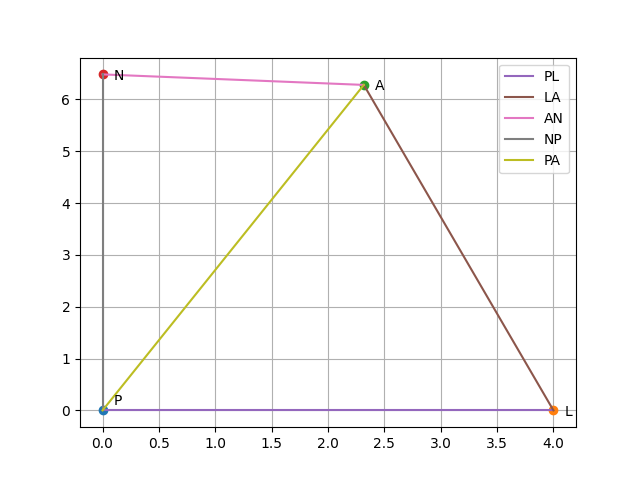
\includegraphics[ width=10cm, height=6 cm]{Quadrilateral_PLAN.png}
    \caption{Quadrilateral PLAN}
    \label{fig:Quadrilateral PLAN}	
\end{figure}  
\end{frame}
\end{document}